
\chapter{绪论}
	\label{chap:introduction}
	\section{研究背景与意义}
	随着物联网和用户终端设备的发展,人们逐渐从信息的匮乏时代走进了信息的过载(Information overload)时代。无论是作为信息消费者的普通用户,还是作为信息生产者的提供商面临着数据爆炸时代的挑战。作为用户,如何从充斥着大量噪声的大数据中找到自己感兴趣的信息是一件非常耗时费力的事情。而作为提供商,如何让自己生产的信息不埋没在大数据洪流中而受到潜在用户的充分关注,这也是其所要解决的一个课题,很多企业已经或者正在开发适合本公司的推荐系统(Recommender System)来解决这一矛盾。笔者曾有过这样的一种购物体验:在淘宝商城购买一台笔记本电脑,花费了一上午的时间才浏览、比较完所有的 thinkpad 品牌商家店面,如\autoref{fig:hl_taobao}。而近年来淘宝的交易额增长规模巨大,2005年淘宝交易额为80亿,2010年为4000亿,而到2015年淘宝双十一单日交易额就为912亿元,可见未来几年内笔者的这种关键字搜索+逐条浏览的购物方式已经不再具有可行性。推荐系统的主要任务就是联系用户和信息,一方面协助用户发现自己潜在感兴趣的信息从而提升用户的满意度,另一方面让信息针对性的展现在只对它有兴趣的用户面前从而提升商品的转化率,于是实现了消费者和生产者的双赢。
	\begin{figure}
		\centering
		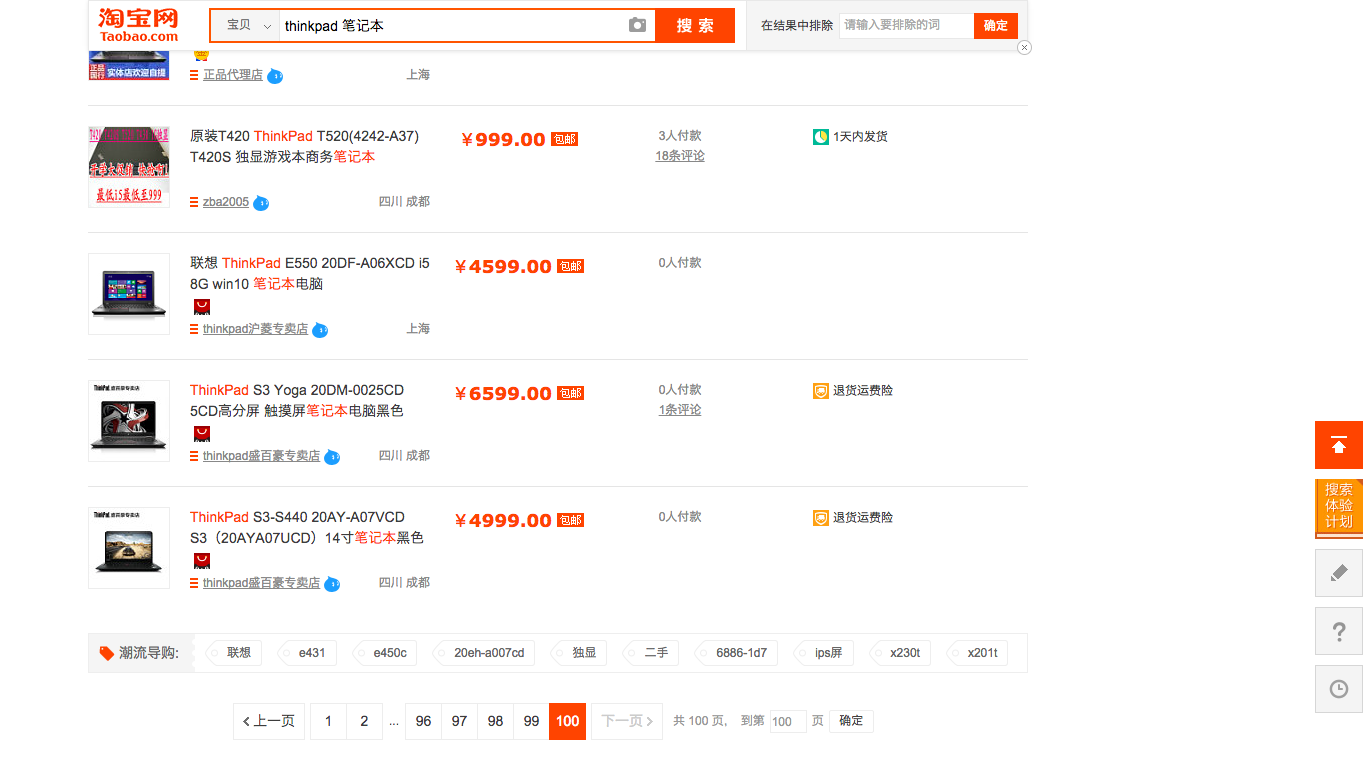
\includegraphics[width=0.9\textwidth]{hl_taobao}
		\figcaption{淘宝购物页面}
		\label{fig:hl_taobao}
	\end{figure}

	自互联网诞生以来,用户寻找信息的方法经历了几个阶段。早期的用户主要靠直接记住感兴趣网站的网址来寻找内容,直接促使Yahoo!提出了分类目录系统,将网站分门别类方便用户查询。但随着信息越来越多,分类目录也只能记录少量的网站,于是产生了搜索引擎。以Google为代表的搜索引擎可以让用户通过关键词找到自己需要的信息,但是,搜索引擎需要用户主动的提供显式关键词来寻找信息,因此它不能解决用户的更多的潜在需求,当用户无法精准描述自己的需求时,搜索引擎就无能为力了,于是又催生出推荐系统\citep{recmd-system}。以亚马逊电商官网为代表的推荐系统是一种帮助用户快速发现有用信息的工具,和搜索引擎不同的是推荐系统不需要提供明确的需求,而是通过分析用户的历史行为来给用户画像建模从而主动给用户推荐出能够满足他们兴趣和需求的信息。因此,从某种意义上说推荐系统和搜索引擎是两个互补的工具。搜索引擎满足用户显式的需求,而推荐系统能够在用户没有明确目的的时候帮助他们发现潜在的需要。

	现有的预测用户兴趣的方法主要有三个。内容过滤(Content Filtering)\citep{content-based}算法认为用户会喜欢和他以前喜欢的物品在内容上相似的物品,比如用户购买了一款基于海贼王的动漫主题包,那么内容过滤算法会给他推荐另一款相似的火影忍者主题包。内容过滤算法主要利用了物品的内容数据,比如主题包的作者,标题,类型,关键词,适用人群等信息。协同过滤(Collaborative Filtering)\citep{collab-filter}不依赖于用户的属性信息和物品的内容信息,而仅仅通过分析大量的用户对物品的行为数据,从社交角度找出特定的相似行为模式,据此来预测用户的兴趣并给用户做出推荐。随着以Tencent和Facebook为代表的社会网络的兴起,社会化过滤(Social Filtering)逐渐成为推荐领域的研究热点。社会化过滤算法\citep{social-filter},认为用户的兴趣和他的好友的兴趣会有共同点,从而可以通过分析用户好友的兴趣来预测给定用户的兴趣。除此之外,还有利用用户年龄,性别,职业,用户地理位置等属性的推荐算法。对于推荐系统来讲,每天都会有大量的新用户加入,老用户离开;大量的新内容上线,旧内容下架,与此同时用户的年龄,兴趣,社会关系,地理位置也会发生变化。因此,时间作为上下文(Context)信息对推荐系统来说是一种重要的要素,对用户的行为有着重要的影响。早期的推荐系统研究对时间相关的动态特性很少涉及,随着很多大时间跨度的商业网站用户行为数据的积累,以及用户画像建模的成熟,越来越多的研发人员开始聚焦、利用用户行为的动态特性。

	基于用户画像的推荐系统可以更好的发掘信息的长尾效应(The Long Tail)。长尾理论\citep{long-tail}指出,电子商务网站相对于传统零售超市的优点是电子商务网站可以给用户提供更多选择的同时,降低了商品流通成本。因为电子商务网站没有货架的成本,增加一个商品只需要在数据库中添加一行商品相关数据而已,但是随着越来越多的商品信息暴露在用户面前,必要会导致用户的不知所措。其实,大数据爆炸式的增长既是挑战也是机遇,如何充分利用大数据驱动运营,是中国互联网企业面临的一个机遇。与长尾效应相对应的是马太效应\citep{matthew-effect},指的是好的越好,坏的越坏,多的越多,少的越少的现象。举一个例,电子商务网站首页的商品列表常常是按照热门商品排列的,一段时间内最热门的商品一定是排在最上边的,由于热门商品列表的长度是有限的,因此那些冷门、小众的商品是不会进入列表。如果用户依赖于这个列表寻找商品,那么进入到这个列表中的商品就会越来越热门,而进入不了这个列表中的商品就会越来越不热门。搜索引擎也有马太效应的问题\citep{matthew-effect:2},在热门搜索词排名靠前的网页会越来越热门,能够获得越来越多的外链,从而在PageRank算法中排名越来越高,也就更容易获得比较高的排名。推荐系统作为一种寻找信息的重要工具,也面临马太效应的挑战\citep{matthew-effect:3}。但是,相比较搜索引擎来讲推荐系统是一个更具有主动性的系统,因此推荐系统能够更好的控制每个商品的展现次数,让长尾商品能够在对其感兴趣的用户面前得到充分的展示。因此,一个好的推荐系统不仅应该能够帮助用户发现有用的信息,而且需要能更好的发掘长尾效应。

	\section{研究内容}
	本文将集中研究推荐系统的用户画像建模和用户兴趣探索模块\citep{user-interest}。利用用户画像、兴趣探索可以改善推荐系统如下几个方面的性能:
		\begin{itemize}
			\item 改善用户冷启动问题:当一个新用户注册生成时,系统一般是对其不了解的,这时可以只给其推荐热门商品,待积累足够用户行为数据时再为其做个性化推荐,但缺点是会加强马太效应。可以利用用户画像中的一些信息,如年龄,性别,职业,用户地理位置作为推荐依据,解决冷启动问题\citep{cold-start}。
			\item 提升推荐系统的时效性:推荐系统的任何在线推荐都要保证在120毫米之内计算完,其中一个解决方案是利用分层思路,即在推荐系统层和服务器日志层之间增加一个用户画像层,如\autoref{fig:hl_construct}所示,通过把一些高难度,复杂性计算的算法放在离线的用户画像建模,提前计算好,在需要被调用的时候,再做一些简单的在线的计算和分装,完成时效性和性能的保证。
			\item 提升推荐系统的安全性:随着电子商务的迅猛发展,商家会通过各种活动形式的补贴来获取用户、培养用户的消费习惯,但同时也催生一些通过刷排行榜、刷红包的用户,严重破环了市场的稳定,侵占了活动的资源。其中一个有效的解决方案就是利用用户画像沉淀方法设置促销活动门槛,即通过记录用户的注册时间、历史登陆次数、常用IP地址等,最大程度上隔离掉僵尸账号,保证市场的稳定发展。
			\item 提升推荐系统的长尾效应:如果用2-8法则来解释的话,就是说百分之20的热门商品占据了百分之80的关注度,百分之80的小众商品只占了百分之20的关注度,即使某用户对某个小众商品有一些高质量的用户行为数据,这些数据也会淹没在太多的热门商品行为数据中,传统的推荐系统不能准确发现这类关联关系。而用户兴趣探索作为专门聚焦于小众兴趣标签的探索,可以提升推荐系统的长尾效应。
		\end{itemize}

		\begin{figure}
			\centering
			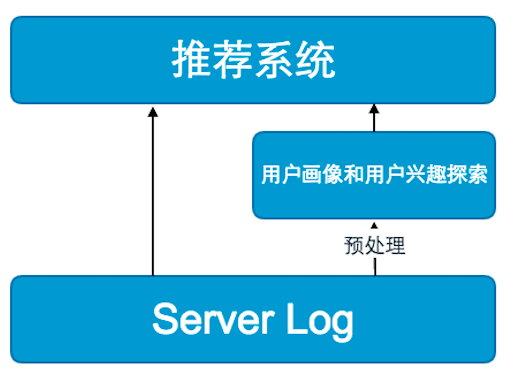
\includegraphics[width=0.5\textwidth]{hl_construct}
			\figcaption{结合了用户画像的推荐系统结构图}
			\label{fig:hl_construct}
		\end{figure}

		\subsection{数据集介绍}
		本文涉及到的数据集主要分为推荐系统的输入数据集和推荐系统的输出数据集。输入数据集由三个不同大小的数据集组成:
		\begin{itemize}
			\item 物品属性向量:用来述一个商品的性质,也经常被称为Item Profile,包括主题名称,作者,上架时间,用户评分,编辑评星,评论,价格,以天为单位的各个时间维度(周,月,年)的下载量和销售量,人工+聚类算法打上的标签等。共包括1.1万个第三方开发的主题包,其中有效主题包有9千多个。
			\item 用户画像 。用来述一个用户的“个性”,也就是User Profile。包括用户注册信息:姓名,年龄,性别,职业,地理位置等,用户活跃度,用户购买力,用户兴趣探索获得的各种兴趣标签及其权重等。数据集包含了300万用户信息,可以用来解决推荐系统的冷启动问题。
			\item 用户行为数据:一般来讲,一个用户在某一时刻对某一个主题包的一次动作算做一条日志,存放在公司的hadoop集群上。用户行为包括显示反馈:浏览,下载,购买,评论,打分,点赞/踩,也包括隐式反馈:停留时长,划屏频率,进入方式等。这个大规模数据集包括了一个月内近5千万条日志,反映了用户对物品的喜好程度。
		\end{itemize}

	\section{论文结构}
	本文的其余正文内容由以下章节组成:
	\begin{itemize}
		\item 第二章首先介绍了现有的推荐系统,包括数据挖掘算法\citep{date-mining}和信息提取技术\citep{info-retrieval}的应用。
		\item 第三章主要讨论了如何利用用户画像解决用户冷启动、用户兴趣多样性的问题,并给出了相关的实验结果及分析。
		\item 第四章主要讨论了如何利用用户兴趣探索跟踪用户动态并挖掘用户小众兴趣,从而提升推荐系统的长尾效应,文中给出了相关的实验结果及分析。
		\item 第五章主要讨论了如何利用A/B test\citep{ab-test}实现人工的特征提取。
		\item 第六章是论文的结束语和展望,在对目前工作简要总结的基础上,提出了推荐系统下一步研究的任务和方向。
	\end{itemize}